% Options for packages loaded elsewhere
\PassOptionsToPackage{unicode}{hyperref}
\PassOptionsToPackage{hyphens}{url}
%
\documentclass[
]{article}
\usepackage{lmodern}
\usepackage{amssymb,amsmath}
\usepackage{ifxetex,ifluatex}
\ifnum 0\ifxetex 1\fi\ifluatex 1\fi=0 % if pdftex
  \usepackage[T1]{fontenc}
  \usepackage[utf8]{inputenc}
  \usepackage{textcomp} % provide euro and other symbols
\else % if luatex or xetex
  \usepackage{unicode-math}
  \defaultfontfeatures{Scale=MatchLowercase}
  \defaultfontfeatures[\rmfamily]{Ligatures=TeX,Scale=1}
\fi
% Use upquote if available, for straight quotes in verbatim environments
\IfFileExists{upquote.sty}{\usepackage{upquote}}{}
\IfFileExists{microtype.sty}{% use microtype if available
  \usepackage[]{microtype}
  \UseMicrotypeSet[protrusion]{basicmath} % disable protrusion for tt fonts
}{}
\makeatletter
\@ifundefined{KOMAClassName}{% if non-KOMA class
  \IfFileExists{parskip.sty}{%
    \usepackage{parskip}
  }{% else
    \setlength{\parindent}{0pt}
    \setlength{\parskip}{6pt plus 2pt minus 1pt}}
}{% if KOMA class
  \KOMAoptions{parskip=half}}
\makeatother
\usepackage{xcolor}
\IfFileExists{xurl.sty}{\usepackage{xurl}}{} % add URL line breaks if available
\IfFileExists{bookmark.sty}{\usepackage{bookmark}}{\usepackage{hyperref}}
\hypersetup{
  pdftitle={Exam 1},
  hidelinks,
  pdfcreator={LaTeX via pandoc}}
\urlstyle{same} % disable monospaced font for URLs
\usepackage[margin=1in]{geometry}
\usepackage{longtable,booktabs}
% Correct order of tables after \paragraph or \subparagraph
\usepackage{etoolbox}
\makeatletter
\patchcmd\longtable{\par}{\if@noskipsec\mbox{}\fi\par}{}{}
\makeatother
% Allow footnotes in longtable head/foot
\IfFileExists{footnotehyper.sty}{\usepackage{footnotehyper}}{\usepackage{footnote}}
\makesavenoteenv{longtable}
\usepackage{graphicx,grffile}
\makeatletter
\def\maxwidth{\ifdim\Gin@nat@width>\linewidth\linewidth\else\Gin@nat@width\fi}
\def\maxheight{\ifdim\Gin@nat@height>\textheight\textheight\else\Gin@nat@height\fi}
\makeatother
% Scale images if necessary, so that they will not overflow the page
% margins by default, and it is still possible to overwrite the defaults
% using explicit options in \includegraphics[width, height, ...]{}
\setkeys{Gin}{width=\maxwidth,height=\maxheight,keepaspectratio}
% Set default figure placement to htbp
\makeatletter
\def\fps@figure{htbp}
\makeatother
\setlength{\emergencystretch}{3em} % prevent overfull lines
\providecommand{\tightlist}{%
  \setlength{\itemsep}{0pt}\setlength{\parskip}{0pt}}
\setcounter{secnumdepth}{-\maxdimen} % remove section numbering

\title{Exam 1}
\author{}
\date{\vspace{-2.5em}}

\begin{document}
\maketitle

\hypertarget{problem-1}{%
\subsection{Problem 1}\label{problem-1}}

Decide the best vertical first split for the following dataset. Impurity
can be measured by entropy or Gini-Index.

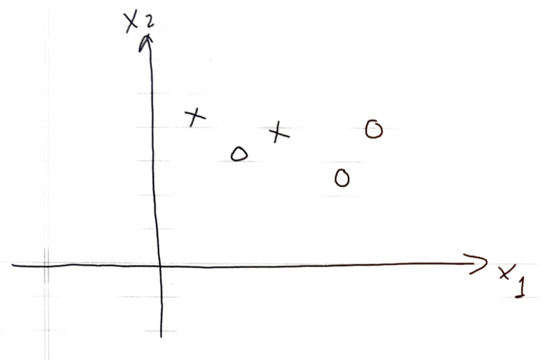
\includegraphics{images/s15.png}

\hypertarget{problem-2}{%
\subsection{Problem 2}\label{problem-2}}

A similar problem and solution can be found here:
\href{Exam1/Exam1.html}{Link}

\begin{itemize}
\tightlist
\item
  Given the \textbf{training} data.
\end{itemize}

\begin{longtable}[]{@{}rrr@{}}
\toprule
Class & Sex & Survived\tabularnewline
\midrule
\endhead
1 & 0 & 1\tabularnewline
1 & 0 & 1\tabularnewline
1 & 0 & 1\tabularnewline
1 & 1 & 1\tabularnewline
1 & 0 & 1\tabularnewline
1 & 0 & 1\tabularnewline
1 & 0 & 1\tabularnewline
3 & 1 & 1\tabularnewline
3 & 0 & 1\tabularnewline
2 & 1 & 0\tabularnewline
3 & 0 & 1\tabularnewline
2 & 1 & 0\tabularnewline
2 & 1 & 0\tabularnewline
3 & 1 & 0\tabularnewline
2 & 1 & 0\tabularnewline
3 & 0 & 0\tabularnewline
1 & 0 & 0\tabularnewline
2 & 0 & 0\tabularnewline
1 & 1 & 0\tabularnewline
2 & 1 & 0\tabularnewline
\bottomrule
\end{longtable}

Using Gini Index as the measure for impurity to:

\begin{enumerate}
\def\labelenumi{\arabic{enumi}.}
\tightlist
\item
  Grow the \textbf{maximum tree} with three leaves (a stopping rule!) on
  the data. Draw the (diagram of) tree.
\item
  Find the misclassification rate on training data of the maximal tree
\item
  Draw all the possible \textbf{subtrees}
\item
  Validate the maximal tree and all the subtrees on the following data
  to select the \textbf{optimal tree}. Note: if the chance of Survived
  is 1/2, predict \texttt{Survived}
\end{enumerate}

\begin{longtable}[]{@{}rrr@{}}
\toprule
Class & Sex & Survived\tabularnewline
\midrule
\endhead
1 & 0 & 1\tabularnewline
1 & 1 & 1\tabularnewline
3 & 1 & 0\tabularnewline
2 & 0 & 0\tabularnewline
\bottomrule
\end{longtable}

\end{document}
